\documentclass[format=acmsmall, review=false, screen=true]{acmart}

\usepackage{booktabs} % For formal tables
\usepackage{multirow}
\usepackage{amsmath}
\usepackage{amssymb}

\usepackage{xr}
\externaldocument{article}

\usepackage[ruled]{algorithm2e} % For algorithms
\renewcommand{\algorithmcfname}{ALGORITHM}
\SetAlFnt{\small}
\SetAlCapFnt{\small}
\SetAlCapNameFnt{\small}
\SetAlCapHSkip{0pt}
\IncMargin{-\parindent}
\setcounter{tocdepth}{4}

\def\thesection{SI-B-\arabic{section}}
\def\thefigure{SI-B-\arabic{figure}}
\def\theequation{SI-B-\arabic{equation}}


% Metadata Information
\acmJournal{CSUR}
\acmVolume{0}
\acmNumber{0}
\acmArticle{0}
\acmYear{0}
\acmMonth{0}
\copyrightyear{2019}
%\acmArticleSeq{9}

% Copyright
%\setcopyright{acmcopyright}
% \setcopyright{acmlicensed}
\setcopyright{rightsretained}
%\setcopyright{usgov}
%\setcopyright{usgovmixed}
%\setcopyright{cagov}
%\setcopyright{cagovmixed}
\acmPrice{0.00}

% DOI
\acmDOI{0000001.0000001}

% Paper history
\received{XXXXX}
\received[revised]{XXXXX}
\received[accepted]{XXXXX}

% \newcommand{\massa}{{\large \textsc{mass}}}
% \newcommand{\mass}{{\large \textsc{mass}}}
% \newcommand{\figgus}{{\large \textsc{figgus}}}
\newcommand{\massa}{MASS}
\newcommand{\mass}{MASS}
\newcommand{\figgus}{MASS}
% Document starts
\begin{document}
% Title portion. Note the short title for running heads 
\title[Spectra of sampled sounds]{Spectra of sampled sounds}  
\author{Renato Fabbri}
% \orcid{1234-5678-9012-3456}
\affiliation{%
  \institution{University of S\~ao Paulo}
  \department{Institute of Mathematics and Computer Sciences}
  \streetaddress{Avenida Trabalhador S\~ao Carlense, 400 - Centro}
  \city{S\~ao Carlos}
  \state{SP}
  \postcode{13566-590}
  \country{Brazil}}
\author{Vilson Vieira da Silva Junior}
\affiliation{%
  \institution{Cod.ai}
%  \department{Research and Development}
  \city{Berlin}
  \state{BE}
  \postcode{???}
  \country{DE}
}
\author{Ant\^onio Carlos Silvano Pessotti}
\affiliation{%
  \institution{Universidade Metodista de Piracicaba}
  \department{??}
  \city{Piracicaba}
  \state{SP}
  \postcode{???}
  \country{Brazil}}
\author{D\'ebora Cristina Corr\^ea}
\affiliation{%
  \institution{University of Western Australia}
  \department{??}
  \city{Piracicaba}
  \state{SP}
  \postcode{???}
  \country{AU}
  }
\author{Osvaldo N. Oliveira Jr.}
\affiliation{%
  \institution{University of S\~ao Paulo}
  \department{S\~ao Carlos Institute of Physics}
  \streetaddress{Avenida Trabalhador S\~ao Carlense, 400 - Centro}
  \city{S\~ao Carlos}
  \state{SP}
  \postcode{13566-590}
  \country{Brazil}
  }

\begin{abstract}
  This Supporting Information document holds an extension of the exposition in the main document to illustrate the spectra os sampled sounds through the components of traditional waveforms with few samples.
\end{abstract}

%
% The code below should be generated by the tool at
% http://dl.acm.org/ccs.cfm
% Please copy and paste the code instead of the example below. 
%
\begin{CCSXML}
  <ccs2012>
    <concept>
      <concept_id>10010405.10010469.10010475</concept_id>
      <concept_desc>Applied computing~Sound and music computing</concept_desc>
      <concept_significance>500</concept_significance>
    </concept>
    <concept>
      <concept_id>10010147.10010341.10010342.10010343</concept_id>
      <concept_desc>Computing methodologies~Modeling methodologies</concept_desc>
      <concept_significance>300</concept_significance>
    </concept>
    <concept>
      <concept_id>10002944.10011122.10002945</concept_id>
      <concept_desc>General and reference~Surveys and overviews</concept_desc>
      <concept_significance>300</concept_significance>
    </concept>
    <concept>
      <concept_id>10002944.10011122.10002946</concept_id>
      <concept_desc>General and reference~Reference works</concept_desc>
      <concept_significance>300</concept_significance>
    </concept>
  </ccs2012>
\end{CCSXML}

\ccsdesc[500]{Applied computing~Sound and music computing}
\ccsdesc[300]{Computing methodologies~Modeling methodologies}
\ccsdesc[300]{General and reference~Surveys and overviews}
\ccsdesc[300]{General and reference~Reference works}

%
% End generated code
%


\keywords{music, acoustics, psychophysics, digital audio, signal processing}


\thanks{This work is supported by FAPESP and CNPq.}


\maketitle

% The default list of authors is too long for headers}
\renewcommand{\shortauthors}{R. Fabbri et al.}

The sinusoidal components in the discretized sound have some particularities.
% no integral and derivatives
Considering a signal $T$ and its corresponding Fourier decomposition 
$\mathcal{F}\langle T\rangle=C=\{c_k\}_0^{\Lambda-1}=\left\{ \sum_{i=0}^{\Lambda-1}t_ie^{-j i (k \frac{2 \pi}{\Lambda})} \right\}_{0}^{\Lambda-1}$,
the recomposition is the sum of the frequency components to yield the temporal samples\footnote{The 
factor $\frac{1}{\Lambda}$ can be distributed among the Fourier transform and its reconstruction, as preferred.
Note that $j$ here is the imaginary unit $j^2=-1$.}:

\begin{equation}\label{recomposicaoFourier}
\begin{split}
t_i = & \frac{1}{\Lambda}\sum_{k=0}^{\Lambda-1}c_ke^{j \frac{2\pi k}{\Lambda} i } \\ 
    = & \frac{1}{\Lambda}\sum_{k=0}^{\Lambda-1}(a_k+ j . b_k)\left[cos(w_k i)   +j . sen(w_k i)\right]
\end{split}
\end{equation}

\noindent where $c_k = a_k + j . b_k$ defines the amplitude and phase of each frequency:
$w_k=\frac{2\pi}{\Lambda}k$ in radians or $f_k=w_k\frac{f_s}{2\pi}=\frac{f_s}{\Lambda}k$ in Hertz,
and are limited by $w_k\leq\pi$ and $f_k\leq\frac{f_s}{2}$ as given by the Nyquist Theorem.

For a sonic signal, samples $t_i$ are real and are given by the real part of Equation~\ref{recomposicaoFourier}:

\begin{equation}\label{moduloEfase}
\begin{split}
t_i& = \frac{1}{\Lambda}\sum_{k=0}^{\Lambda-1}\left[a_k cos(w_k i) -b_k sen(w_k i)\right] \\
	& = \frac{1}{\Lambda}\sum_{k=0}^{\Lambda-1}\sqrt{a_k^2 + b_k^2} \; cos\left[w_k i - arctan(b_k, a_k)\right]
\end{split}
\end{equation}

\noindent where $arctan(x, y) \in [0, 2\pi]$ is the inverse tangent with the right choice of the quadrant
in the imaginary plane.

$\Lambda$ real samples $t_i$ result in $\Lambda$ complex coefficients $c_k=a_k+j.b_k$.
The coefficients $c_k$ are equivalent two by two,
corresponding to the same frequencies and with the same contribution to its reconstruction.
They are complex conjugates: $a_{k1}=a_{k2}$ and $b_{k1}=-b_{k2}$ and, as a consequence, the modules are equal and phases have opposite signs.
Recalling that $f_k = k\frac{f_s}{\Lambda}, \; k \in \left\{0, ..., \left \lfloor \frac{\Lambda}{2} \right \rfloor \right\} $.
When $k > \frac{\Lambda}{2}$, the frequency $f_k$ is mirrored through $\frac{f_s}{2}$ in this way: $f_k=\frac{f_s}{2} - (f_k-\frac{f_s}{2})=f_s-f_k=f_s - k\frac{f_s}{\Lambda}=(\Lambda-k)\frac{f_s}{\Lambda} \;\;\;\; \Rightarrow \;\;\;\; f_k\equiv f_{\Lambda-k} \; ,\;\; \forall \;\; k<\Lambda$.

The same applies to $w_k=f_k\frac{2\pi}{f_s}$ and the periodicity $2\pi$:
it follows that $w_k=-w_{\Lambda-k} \; ,\;\; \forall \;\; k<\Lambda$.
Given the cosine (an even function) and the inverse tangent (an odd function),
the components in $w_k$ and $w_{\Lambda-k}$ contribute with coefficients $c_k$ = $c^*_{\Lambda-k}$ in the reconstruction of the real samples.
In summary, in a decomposition of $\Lambda$ samples, the $\Lambda$ frequency components $\{c_i\}_0^{\Lambda-1}$ are equivalent in pairs,
except for $f_0$, and, when $\Lambda$ is even, for $f_{\Lambda/2}=f_{\text{max}}=\frac{f_s}{2}$.
Both these components are isolated, i.e.\ there is one and only one component at frequency $f_0$ or $f_{\Lambda/2}$ (if $\Lambda$ is even).
In fact, when $k=0$ or $k=\Lambda/2$ the mirror of the frequencies are themselves: $f_{\Lambda/2}=f_{(\Lambda-\Lambda/2) = \Lambda/2}$ and $f_0=f_{(\Lambda-0)=\Lambda}=f_0$.
Furthermore, these two frequencies (zero and Nyquist frequency) do not have a phase offset: their coefficients are strictly real.
Therefore, the number $\tau_\Lambda$ of equivalent coefficient pairs in a decomposition of $\Lambda$ samples is:

\begin{equation}\label{coefsPareados}
	\tau_\Lambda = \frac{\Lambda - \Lambda \% 2}{2} -2 +\Lambda \% 2 = \left \lceil \frac{\Lambda}{2} \right \rceil -2
\end{equation}

This discussion can be summarized in the following equivalences:

\begin{align}
	f_{k}\equiv f_{\Lambda-k}& \;\; , \;\; w_{k}\equiv-w_{\Lambda-k} \label{equivalenciasFreqs} \\
	 a_k = a_{\Lambda -k}& \;\; , \;\;b_k = - b_{\Lambda -k} \label{equavalenciasTermos} \\
	\sqrt{a_k^2 + b_k^2} & = \sqrt{a_{\Lambda - k}^2 + b_{\Lambda -k}^2}\label{equivalenciasModulos} \\
	arctan(b_k, a_k) & = -arctan(b_{\Lambda -k}, a_{\Lambda - k}) \label{equivalenciasFases}
\end{align}

\noindent with
$\forall \; 1 \leq k \leq \tau_\Lambda$, 
$k \in \mathbb{N}$.

To express the general case for components combination in each sample $t_i$,
one can gather the relations for the reconstruction of a real signal (Equation~\ref{moduloEfase}),
for the number of paired coefficients (Equation~\ref{coefsPareados}),
and for the equivalences of modules (Equation~\ref{equivalenciasModulos})
and phases (Equation~\ref{equivalenciasFases}):

\begin{equation}\label{eq:reconsCompleta}
\begin{split}
	t_i = \frac{a_0}{\Lambda} + \frac{ a_{\Lambda/2}}{\Lambda}(1-\Lambda\% 2) + \frac{2}{\Lambda}\sum_{k=1}^{\tau_\Lambda}\sqrt{a_k^2 + b_k^2} \; cos\left[w_k i - arctan(b_k,a_k)\right]
\end{split}
\end{equation}

 \begin{figure*}
     \centering
         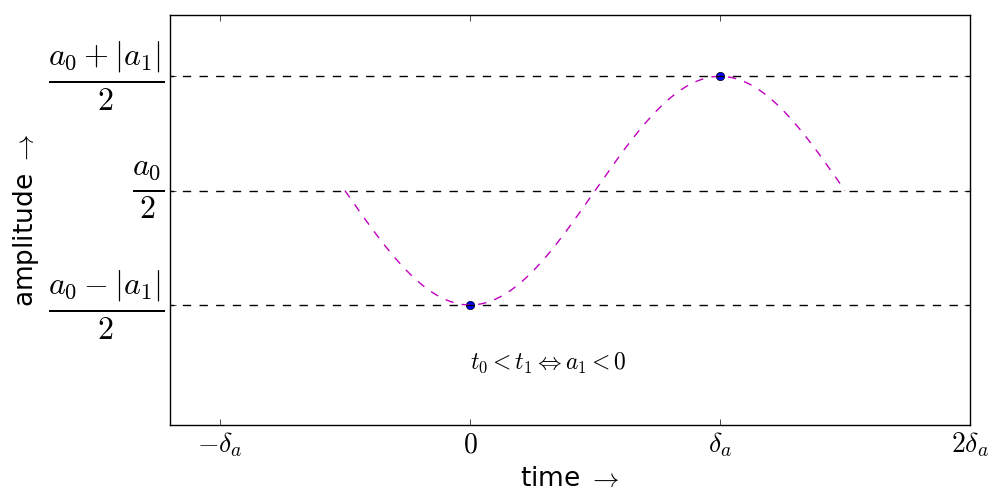
\includegraphics[width=.7\textwidth]{figures/amostras2c___}
	 \caption{Oscillation of 2 samples (maximum frequency for any $f_s$). The first coefficient determines a constant detachment (called \emph{offset}, \emph{bias} or \emph{DC component}) and the second coefficient specifies the oscillation amplitude.}
         \label{fig:amostras2}
 \end{figure*}

Figure~\ref{fig:amostras2} shows two samples and their spectral component. When there is only two samples, the Fourier decomposition has only one pair of coefficients $\{c_k=a_k-j.b_k\}_0^{\Lambda-1=1}$ relative to frequencies $\{f_k\}_0^1=\left\{w_k\frac{f_s}{2\pi}\right\}_0^1=\left\{k\frac{f_s}{\Lambda=2}\right\}_0^1=\left\{0,\frac{f_s}{2}=f_{\text{max}}\right\}$
with energies $e_k=\frac{(c_k)^2}{\Lambda=2}$. The role of amplitudes $a_k$ is clearly observed with $\frac{a_0}{2}$, the fixed offset (also called \emph{bias} or \emph{DC component}), and $\frac{a_1}{2}$ for the oscillation with frequency $f_1=\frac{f_s}{\Lambda=2}$.
This case has special relevance: at least 2 samples are necessary to represent an oscillation and it yields the Nyquist frequency $f_{\text{max}}=\frac{f_s}{2}$, which is the maximum frequency in a sound sampled with $f_s$ samples per second.

All fixed sequences $T$ of only $3$ samples also have just $1$ frequency, since the first harmonic would have $1.5$ samples and exceeds the bottom limit of 2 samples, i.e.\ the frequency of the harmonic would exceed the Nyquist frequency:  $\; \frac{2. f_s}{3} > \frac{f_s}{2}$. 
The coefficients $\{c_k\}_0^{\Lambda-1=2}$ are present in 3 frequency components. One is relative to frequency zero ($c_0$), and the other two ($c_1$ and $c_2$) have the same role for reconstructing a sinusoid with $f=f_s/3$.
This case is illustrated in Figure~\ref{fig:amostras3}.

 \begin{figure*}
     \centering
         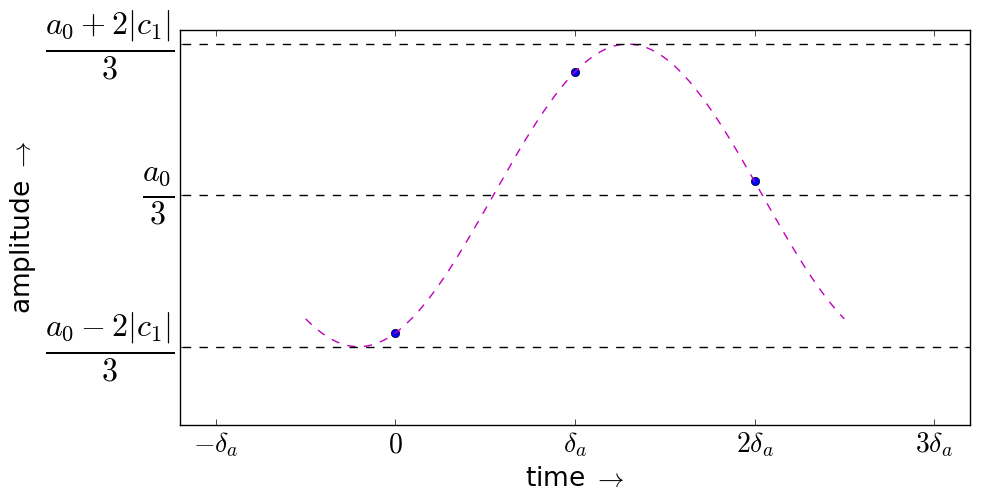
\includegraphics[width=.7\textwidth]{figures/amostras3b_}
     \caption{Three fixed samples present only one non-null frequency. $c_1=c_2^*$ and $w_1 \equiv w_2$.}
         \label{fig:amostras3}
 \end{figure*}

\begin{figure*}
    \centering
        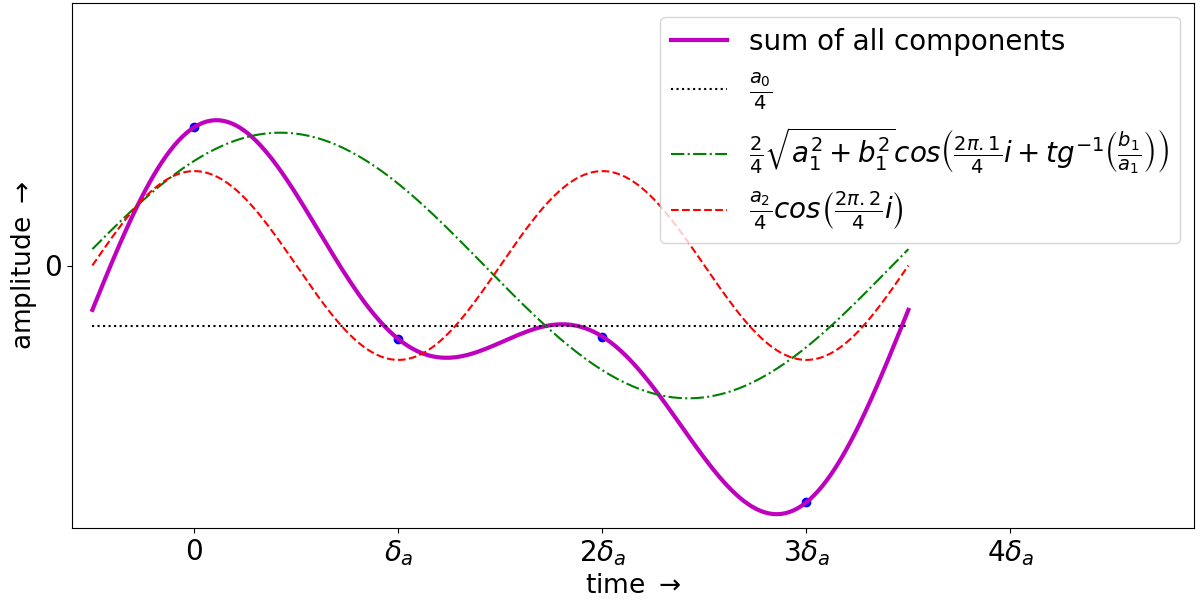
\includegraphics[width=.7\textwidth]{figures/amostras4____}
    \caption{Frequency components for 4 samples.}
        \label{fig:amostras4}
\end{figure*}


\begin{figure*}
    \centering
        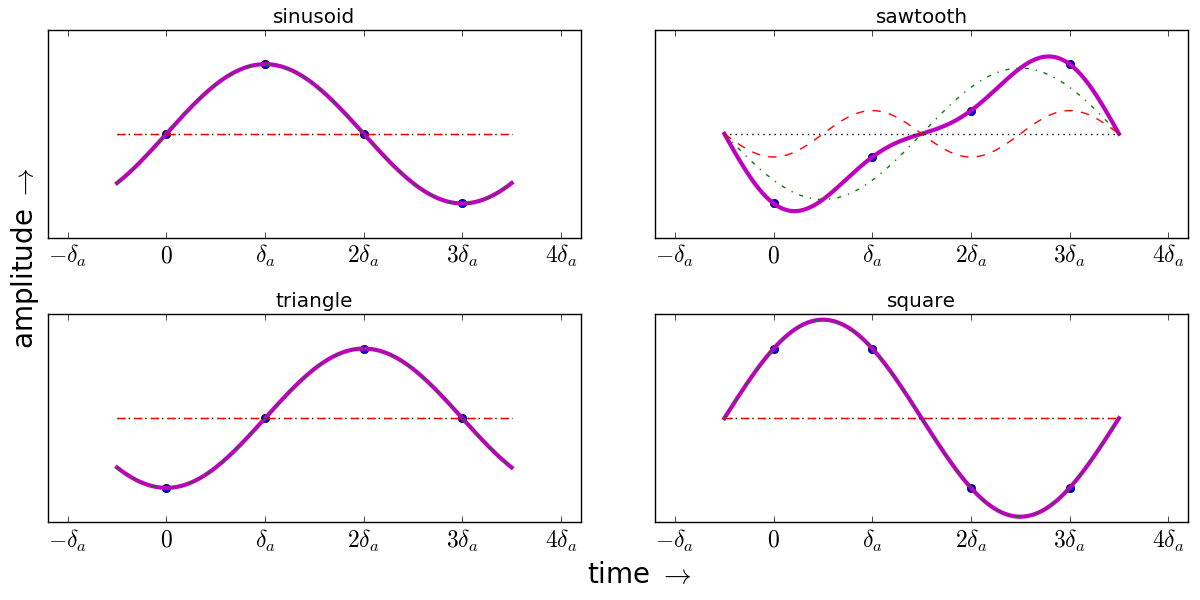
\includegraphics[width=.9\textwidth]{figures/amostras4formas___}
    \caption{Basic waveforms with 4 samples.}
        \label{fig:formas4}
\end{figure*}

\begin{figure*}[!h!]
    \centering
        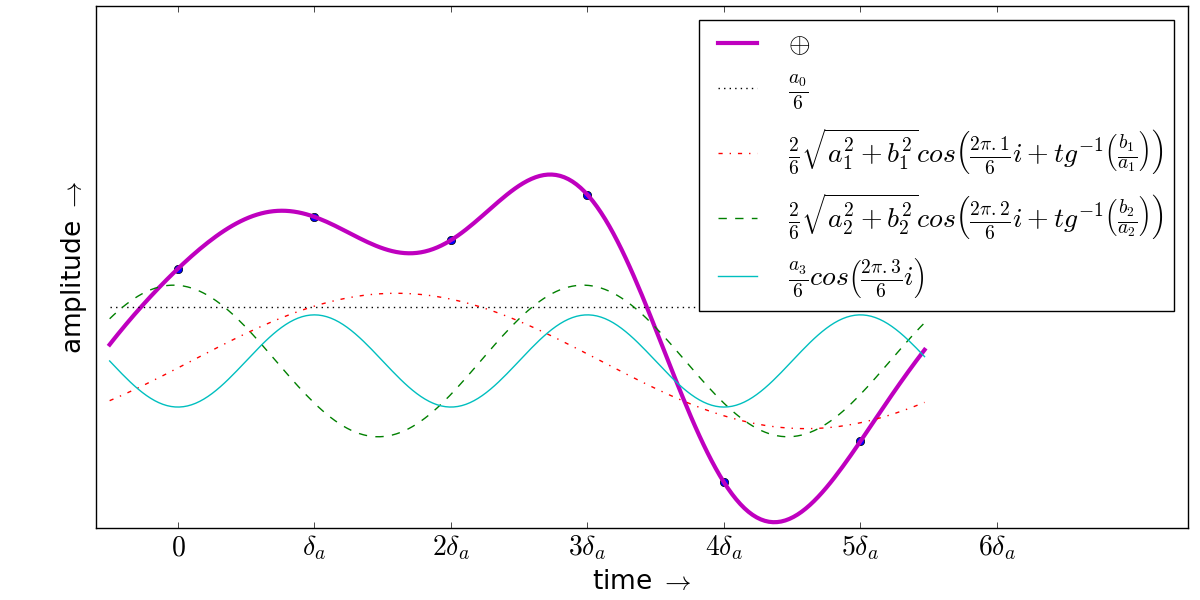
\includegraphics[width=.7\textwidth]{figures/amostras6__}
    \caption{Frequency components for 6 samples: 4 sinusoids, one of them is the \emph{bias} with zero frequency.}
        \label{fig:amostras6}
\end{figure*}

With 4 samples it is possible to represent 1 or 2 frequencies with independence of magnitude and phase.
Figure~\ref{fig:amostras4} depicts the contribution of each of the two (possible) components.
The individual components sum to the original waveform and a brief inspection reveals 
the major curvatures resulting from the higher frequency,
while the fixed offset is captured in the component with frequency $f_0=0$.
Figure~\ref{fig:formas4} shows the harmonics for the basic waveforms of 
Equations~\ref{sinusoid},~\ref{sawTooth},~\ref{triangular} and~\ref{square}
in the case of 4 samples.
There is only 1 sinusoid for each waveform, with the exception of the sawtooth, which has the even harmonics.

\begin{figure*}[!h!]
    \centering
        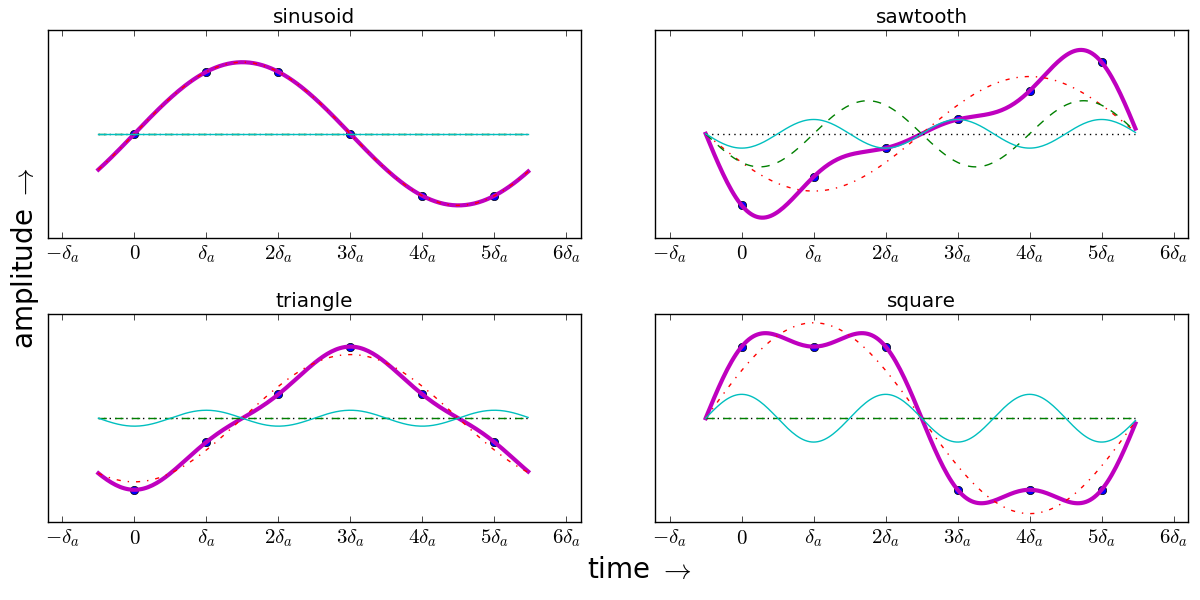
\includegraphics[width=.9\textwidth]{figures/amostras6formas___}
    \caption{Basic waveforms with 6 samples: triangular and square waveforms have odd harmonics, with different proportions and phases; the sawtooth has even harmonics.}
        \label{fig:formas6}
\end{figure*}

Figure~\ref{fig:amostras6} exposes the sinusoidal components within 6 samples,
while Figure~\ref{fig:formas6} presents the decomposition of the basic waveforms:
square and triangular have the same components but in different proportions, while the sawtooth has an extra component.


% \bibliography{sample-bibliography}
% \bibliographystyle{ACM-Reference-Format}
% \bibliography{./article2}
\end{document}
